\documentclass[14pt,t]{beamer-accessibility}
\usetheme{Boadilla}
\usepackage{tikz}
\begin{document}
\begin{frame}{Histogram Figure}
\begin{center}
\begin{accessibleFigure}[alt={Histogram showing main cluster from 25 to 32 percent with peak frequency in center.}]

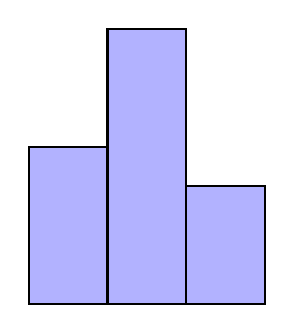
\begin{tikzpicture}
\draw[thick, fill=blue!30] (0,0) rectangle (1,2);
\draw[thick, fill=blue!30] (1,0) rectangle (2,3.5);
\draw[thick, fill=blue!30] (2,0) rectangle (3,1.5);
\end{tikzpicture}
\end{accessibleFigure}
\end{center}
\end{frame}
\end{document}
